\chapter{Logic Optimisation with Karnaugh Maps}\label{ch:kmap}

\begin{objectives}
After studying this chapter you will be able to:
\begin{itemize}
  \item draw two-, three- and four-variable Karnaugh maps and plot a function on them;
  \item find all prime implicants, identify the essential ones, and derive a minimal sum-of-products (SOP) expression;
  \item exploit don't-care conditions to obtain simpler circuits;
  \item derive a minimal product-of-sums (POS) expression by grouping the 0s;
  \item implement SOP and POS expressions with two-level NAND--NAND and NOR--NOR circuits, and explain why NAND and NOR are universal gates;
  \item use XOR and XNOR gates, recognise odd and even functions, and design parity generators and checkers.
\end{itemize}
\end{objectives}

\section{The Need for Optimisation}
In the design flow of \cref{fig:comb-flow}, the step after deriving a Boolean expression from a truth table (for example with minterms, \cref{sec:synthesis}) is \emph{optimisation}. A simpler expression gives a circuit with fewer gates, which is cheaper, usually faster and consumes less power. Algebraic manipulation, as in \cref{ex:simplify}, can do the job, but it follows no fixed rule: it is not obvious which identity to apply next, nor when to stop. The \term{Karnaugh map} turns simplification into a pattern-recognition task that a person can perform reliably for up to about five variables.

\figside{540.1pt}{lect_3_combinational_design_flow}{Design flow of a combinational circuit: specification, truth table, Boolean expression, optimisation and implementation.}{fig:comb-flow}

\section{The Karnaugh Map}
The Karnaugh map (K-map), introduced by Maurice Karnaugh in 1953~\cite{karnaugh1953}, is a pictorial form of the truth table. It is a diagram made up of squares, \emph{each square representing one minterm}. It is arranged so that squares that are \emph{adjacent}, horizontally or vertically, represent minterms that differ in exactly one variable. Two such minterms can be combined by the combining identity $xy+xy'=x$, which removes the variable that changes. The map thus displays, at a glance, all the pairs of minterms that can be merged.

\figw{180.0pt}{lect_3_kmap_example}{A Karnaugh map is a truth table rearranged so that neighbouring squares differ in one variable.}{fig:kmap-example}

\subsection{The two-variable map}
A function of two variables has $2^2=4$ minterms, so its map has four squares (\cref{fig:kmap2}). The rows correspond to the values of $x$ and the columns to the values of $y$. To plot a function, write a 1 in the square of every minterm of the function. For instance $f=xy$ is the single minterm $m_3$, while $f=x+y=m_1+m_2+m_3$ has three 1s.

\begin{figure}[htbp]
\centering
\begin{subfigure}[b]{128.7pt}\centering
  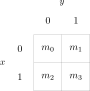
\includegraphics[width=126.7pt]{lect_3_kmap_2var_minterm}\caption{minterms}
\end{subfigure}
\hfill
\begin{subfigure}[b]{128.7pt}\centering
  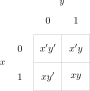
\includegraphics[width=126.7pt]{lect_3_kmap_2var_variable}\caption{variables}
\end{subfigure}
\hfill
\begin{subfigure}[b]{128.7pt}\centering
  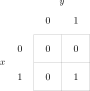
\includegraphics[width=126.7pt]{lect_3_kmap_x_and_y}\caption{$f=xy$}
\end{subfigure}
\\[6pt]
\begin{subfigure}[b]{128.7pt}\centering
  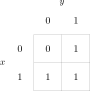
\includegraphics[width=126.7pt]{lect_3_kmap_x_or_y}\caption{$f=x+y$}
\end{subfigure}
\caption{Two-variable K-maps: the layout of minterms and variables, and two plotted functions.}\label{fig:kmap2}
\end{figure}

\subsection{The three-variable map}
Three variables give $2^3 = 8$ squares, arranged in two rows and four columns (\cref{fig:kmap3}). The key point is that the columns are ordered in \term{Gray code}, $00, 01, 11, 10$, not in binary order: in a Gray code only one bit changes between consecutive code words. Because of this, horizontally adjacent squares differ in exactly one variable. The ordering also makes the \emph{leftmost and rightmost columns adjacent}, as if the map were wrapped around a cylinder (column $10$ is adjacent to column $00$).

Two adjacent 1s can be merged to remove one variable. For example $m_5$ and $m_7$ are adjacent: $xy'z + xyz = xz(y'+y) = xz$.

\figw{180.0pt}{lect_3_kmap_3var_structure}{Structure of the three-variable K-map. Columns follow a Gray code and wrap around.}{fig:kmap3}

\subsection{Rules for simplification}
\begin{keypoint}[Rules for grouping on a K-map]
The aim is to cover all the 1s of the map with as few and as large groups as possible.
\begin{enumerate}
  \item Groups must be \textbf{rectangles} containing $1, 2, 4, 8,\dots$ squares (a power of two).
  \item Make each group \textbf{as large as possible}; a group of four is better than two groups of two.
  \item \textbf{Every 1 must be covered} by at least one group.
  \item Groups \textbf{may overlap} if this allows larger groups.
  \item \textbf{Wrap-around} adjacency is allowed: the left and right edges, and the top and bottom edges, are neighbours.
  \item Use the \textbf{fewest groups} that cover all the 1s.
\end{enumerate}
Each group gives one product term; the variables that take a constant value over the whole group appear in the term (uncomplemented if the constant is 1, complemented if it is 0) and the variables that change are eliminated. The simplified function is the OR of the product terms. A group of $2^k$ squares eliminates $k$ variables.
\end{keypoint}

\begin{example}{Two groups of two}{kmap1}
Simplify $F(x,y,z)=\Sm(2,3,4,5)$.

\textbf{Solution.} Plot 1s in squares 2, 3, 4 and 5 (\cref{fig:ex31}). Minterms $m_2,m_3$ ($x'yz'$ and $x'yz$) are adjacent and combine to $x'y$; $m_4,m_5$ ($xy'z'$ and $xy'z$) combine to $xy'$. Hence
\[ F = x'y + xy' = x\xor y. \]
\end{example}

\begin{example}{Groups with wrap-around}{kmap2}
Simplify $F(x,y,z)=\Sm(3,4,6,7)$.

\textbf{Solution.} $m_3$ and $m_7$ ($x'yz$, $xyz$) combine to $yz$. $m_4$ and $m_6$ ($xy'z'$, $xyz'$) are adjacent \emph{through the wrap-around} (column $00$ to column $10$) and combine to $xz'$. Hence $F = yz + xz'$ (\cref{fig:ex32}).
\end{example}

\begin{example}{A group of four}{kmap3}
Simplify $F(x,y,z)=\Sm(0,2,4,6)$.

\textbf{Solution.} All four 1s form a single group (the two outer columns, joined by wrap-around). Over this group $x$ takes both values and so does $y$, so both are eliminated; $z$ is 0 in all four squares, so $z'$ remains: $F = z'$ (\cref{fig:ex33}). A group of four eliminates two variables.
\end{example}

\begin{example}{Overlapping groups}{kmap4}
Simplify $F(x,y,z)=\Sm(0,2,4,5,6)$.

\textbf{Solution.} The largest group covers $m_0,m_2,m_4,m_6$ and gives $z'$. The 1 in $m_5$ is not yet covered; the largest group containing it is $m_4,m_5$, which gives $xy'$. Note that $m_4$ belongs to both groups, which is allowed and gives the simplest result: $F = z' + xy'$ (\cref{fig:ex34}).
\end{example}

\begin{figure}[htbp]
\centering
\begin{subfigure}[b]{182.0pt}\centering
  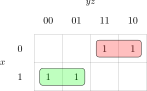
\includegraphics[width=180.0pt]{kmap_3var_ex1}\caption{\cref{ex:kmap1}}\label{fig:ex31}
\end{subfigure}
\hfill
\begin{subfigure}[b]{182.0pt}\centering
  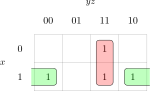
\includegraphics[width=180.0pt]{lect_3_kmap_3var_ex2}\caption{\cref{ex:kmap2}}\label{fig:ex32}
\end{subfigure}
\\[6pt]
\begin{subfigure}[b]{182.0pt}\centering
  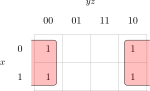
\includegraphics[width=180.0pt]{lect_3_kmap_3var_ex3}\caption{\cref{ex:kmap3}}\label{fig:ex33}
\end{subfigure}
\hfill
\begin{subfigure}[b]{182.0pt}\centering
  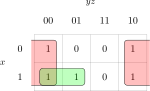
\includegraphics[width=180.0pt]{kmap_3var_ex4}\caption{\cref{ex:kmap4}}\label{fig:ex34}
\end{subfigure}
\caption{K-maps for \cref{ex:kmap1,ex:kmap2,ex:kmap3,ex:kmap4}.}\label{fig:ex3x}
\end{figure}

\section{Prime Implicants}
The grouping procedure can be stated more precisely with three definitions.

\begin{definition}{Implicants}{implicant}
An \term{implicant} of a function is a product term that covers one or more minterms of the function (every group of 1s on the map is an implicant). A \term{prime implicant} (PI) is an implicant that cannot be combined with another to form a larger implicant, that is, a group of 1s that is as large as it can be. An \term{essential prime implicant} (EPI) is a prime implicant that covers at least one minterm covered by no other prime implicant.
\end{definition}

\begin{keypoint}[Minimisation procedure]
\begin{enumerate}
  \item Find all prime implicants.
  \item Include all essential prime implicants.
  \item Choose the smallest set of the remaining prime implicants that covers all the 1s not yet covered.
\end{enumerate}
\end{keypoint}

\section{The Four-Variable Map}
A function of four variables has 16 minterms and a $4\times4$ map (\cref{fig:kmap4}). Both the rows (variables $w,x$) and the columns (variables $y,z$) are in Gray-code order $00,01,11,10$. Wrap-around applies in both directions: the top row is adjacent to the bottom row, and the left column to the right column; in effect the map is a torus. The four corners are therefore adjacent to one another.

\figw{186.2pt}{lect_3_kmap_4x4_structure}{Structure of the four-variable K-map.}{fig:kmap4}

\begin{example}{Four-variable simplification}{kmap5}
Simplify $F(w,x,y,z)=\Sm(0,1,2,4,5,6,8,9,12,13,14)$.

\textbf{Solution.} The map is \cref{fig:ex35}. Look for the largest groups first.
\begin{itemize}
  \item The eight squares in the two columns where $y=0$ (minterms 0, 1, 4, 5, 8, 9, 12, 13) form a group of eight: the term is $y'$.
  \item $m_0,m_2,m_4,m_6$ form a group of four (using the wrap-around between columns $00$ and $10$): $w'z'$.
  \item $m_4,m_6,m_{12},m_{14}$ form a group of four (again by wrap-around): $xz'$.
\end{itemize}
All eleven 1s are covered, and each group is needed ($y'$ is the only group containing $m_1,m_9$; $w'z'$ is the only one containing $m_2$; $xz'$ is the only one containing $m_{14}$). Hence
\[ F = y' + w'z' + xz'. \]
\end{example}

\begin{example}{More than one minimal expression}{kmap6}
Simplify $F(A,B,C,D)=\Sm(0,1,2,5,7,8,9,10,13,15)$.

\textbf{Solution.} The prime implicants are $B'C'$ ($m_0,m_1,m_8,m_9$), $B'D'$ ($m_0,m_2,m_8,m_{10}$), $BD$ ($m_5,m_7,m_{13},m_{15}$) and $C'D$ ($m_1,m_5,m_9,m_{13}$). $B'D'$ is essential because it alone covers $m_2$ and $m_{10}$, and $BD$ is essential because it alone covers $m_7$ and $m_{15}$. The essential prime implicants cover all the 1s except $m_1$ and $m_9$, and either of the remaining prime implicants covers both. There are therefore \emph{two} minimal expressions (\cref{fig:ex36}):
\[ F = BD + B'D' + B'C' \qquad\text{or}\qquad F = BD + B'D' + C'D. \]
They have the same cost; the choice may depend on which signals are already available.
\end{example}

\begin{figure}[htbp]
\centering
\begin{subfigure}[b]{188.2pt}\centering
  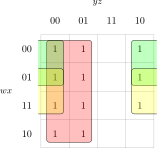
\includegraphics[width=186.2pt]{lect_3_kmap_4x4_ex5}\caption{\cref{ex:kmap5}}\label{fig:ex35}
\end{subfigure}
\hfill
\begin{subfigure}[b]{190.2pt}\centering
  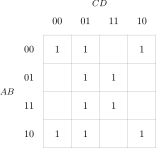
\includegraphics[width=188.2pt]{lect_3_kmap_4x4_ex6_1}\caption{plotted $F$}
\end{subfigure}
\\[6pt]
\begin{subfigure}[b]{190.2pt}\centering
  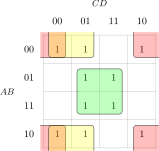
\includegraphics[width=188.2pt]{lect_3_kmap_4x4_ex6_sol_1}\caption{solution 1}
\end{subfigure}
\hfill
\begin{subfigure}[b]{190.2pt}\centering
  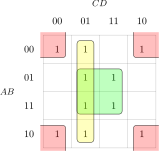
\includegraphics[width=188.2pt]{lect_3_kmap_4x4_ex6_sol_2}\caption{solution 2}
\end{subfigure}
\caption{(a)~\Cref{ex:kmap5}. (b--d)~\Cref{ex:kmap6}: the map and its two minimal covers.}\label{fig:ex36}
\end{figure}

\section{Don't-Care Conditions}\label{sec:dontcare}
In many designs the output for some input combinations is not specified. These are \term{don't-care conditions}. They arise because (a)~the input combination can never occur (for example, the six invalid codes $1010$ to $1111$ of a 4-bit BCD input), or (b)~the output for that input does not matter. On the map a don't-care is marked with an \textbf{X} (sometimes ``d''). The rules are:
\begin{itemize}
  \item treat an X as a 1 if this lets you form a larger group;
  \item otherwise treat it as a 0 (ignore it);
  \item you need \emph{not} cover all the X squares.
\end{itemize}

\begin{example}{Using don't-cares}{dontcare}
Simplify $F(w,x,y,z) = \Sm(1,3,7,11,15) + d(0,2,5)$.

\textbf{Solution.} See \cref{fig:dontcare}. The group $m_3,m_7,m_{11},m_{15}$ gives $yz$. The remaining 1, $m_1$, can be grouped with the don't-cares in two ways: $m_1,m_3,m_5,m_7$ gives $w'z$, and $m_0,m_1,m_2,m_3$ gives $w'x'$. Either is acceptable:
\[ F = yz + w'z \qquad\text{or}\qquad F = yz + w'x'. \]
Without don't-cares, $m_1$ could be combined only with $m_3$, giving a less simple term $w'x'z$.
\end{example}

\figw{357.4pt}{lect_3_kmap_dontcare}{K-map with don't-care conditions for \cref{ex:dontcare}.}{fig:dontcare}

\section{Five- and Six-Variable Maps}
For more than four variables the method still works but becomes harder to apply. A \textbf{five-variable} map consists of two four-variable maps, one for $a=0$ and one for $a=1$, imagined to be stacked (\cref{fig:kmap56}a). Squares are adjacent if they are adjacent within one four-variable map \emph{or} are in the same position in the two maps; thus $m_0$ and $m_{16}$ are adjacent. A \textbf{six-variable} map has four such maps, arranged in a $2\times2$ grid according to $ab$ (\cref{fig:kmap56}b). Beyond six variables, a K-map is no longer practical, and tabular methods such as the \term{Quine--McCluskey algorithm}~\cite{mccluskey1956}, which can be programmed, are used; the logic-synthesis tools used in practice are based on more efficient heuristics of the same kind.

\begin{figure}[htbp]
\centering
\begin{subfigure}[b]{294.1pt}\centering
  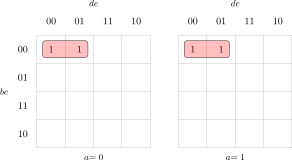
\includegraphics[width=292.1pt]{lect_3_kmap_5var}\caption{five variables}
\end{subfigure}
\caption{K-maps for five and six variables.}\label{fig:kmap56}
\end{figure}

\begin{figure}[htbp]
\centering
\ContinuedFloat
\begin{subfigure}[b]{294.8pt}\centering
  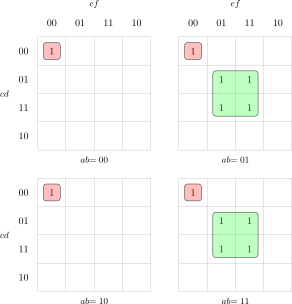
\includegraphics[width=292.8pt]{lect_3_kmap_6var}\caption{six variables}
\end{subfigure}
\caption[]{K-maps for five and six variables.}
\end{figure}

\section{Product-of-Sums Simplification}
A K-map also yields a minimal POS expression: \emph{group the 0s} instead of the 1s. There are two equivalent methods.

\paragraph{Method 1: simplify $F'$ and complement.} Group the 0s of $F$ (the 1s of $F'$) to obtain a minimal SOP for $F'$, then apply De~Morgan's theorem: if $F'=AB+C'D$, then $F=(AB+C'D)'=(A'+B')(C+D')$.

\paragraph{Method 2: direct.} For each group of 0s write a \emph{sum} term: a variable that is 0 over the group appears uncomplemented, a variable that is 1 appears complemented, and a variable that changes is eliminated. The function is the product of the sum terms.

\begin{example}{POS from a K-map}{pos}
Find the minimal POS of $F(A,B,C,D)=\Sm(0,1,2,5,8,9,10)$.

\textbf{Solution.} The 0s are at $m_3,m_4,m_6,m_7,m_{11},m_{12},m_{13},m_{14},m_{15}$ (\cref{fig:pos}). Group them as follows.
\begin{itemize}
  \item $m_{12},m_{13},m_{14},m_{15}$: $A=1,B=1$, giving the sum $(A'+B')$.
  \item $m_3,m_7,m_{11},m_{15}$: $C=1,D=1$, giving $(C'+D')$.
  \item $m_4,m_6,m_{12},m_{14}$: $B=1$, $D=0$, giving $(B'+D)$.
\end{itemize}
Hence $F=(A'+B')(C'+D')(B'+D)$.
\end{example}

\figw{188.2pt}{lect_3_kmap_pos}{Grouping the 0s of \cref{ex:pos}.}{fig:pos}

\section{NAND and NOR as Universal Gates}
The NAND gate ($(xy)'$) and the NOR gate ($(x+y)'$) are called \term{universal gates}: every other gate can be built from NANDs alone, or from NORs alone, so any digital circuit can be built from just one type of gate. This is useful because in many technologies NAND and NOR gates are smaller and faster than AND and OR gates. \Cref{fig:universal} shows the constructions; each follows from De~Morgan's theorem. A NAND with its inputs tied together is a NOT: $(xx)'=x'$. An AND is a NAND followed by a NAND used as an inverter. An OR is built from inverted inputs: $x+y=(x'y')'$. The NOR constructions are the duals.

\begin{figure}[htbp]
\centering
\begin{subfigure}[b]{130.0pt}\centering
  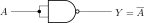
\includegraphics[width=128.0pt]{lect_3_nand_as_not}\caption{NOT}
\end{subfigure}
\hfill
\begin{subfigure}[b]{183.5pt}\centering
  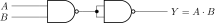
\includegraphics[width=181.5pt]{lect_3_nand_as_and}\caption{AND}
\end{subfigure}
\\[6pt]
\begin{subfigure}[b]{208.5pt}\centering
  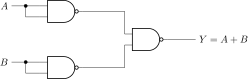
\includegraphics[width=206.5pt]{lect_3_nand_as_or}\caption{OR}
\end{subfigure}
\hfill
\begin{subfigure}[b]{144.9pt}\centering
  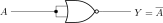
\includegraphics[width=142.9pt]{lect_3_nor_as_not}\caption{NOT}
\end{subfigure}
\\[6pt]
\begin{subfigure}[b]{187.2pt}\centering
  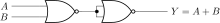
\includegraphics[width=185.2pt]{lect_3_nor_as_or}\caption{OR}
\end{subfigure}
\hfill
\begin{subfigure}[b]{204.7pt}\centering
  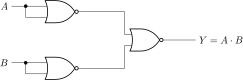
\includegraphics[width=202.7pt]{lect_3_nor_as_and}\caption{AND}
\end{subfigure}
\caption{Universal gates: NOT, AND and OR built from NAND gates only (top row) or from NOR gates only (bottom row).}\label{fig:universal}
\end{figure}

\subsection{Two-level NAND--NAND implementation of an SOP}
A minimal SOP expression is normally drawn as a two-level AND--OR circuit. Applying De~Morgan's theorem to the double complement converts it directly to \emph{two levels of NAND gates}:
\[
 F = AB + CD + E = \bigl((AB+CD+E)'\bigr)' = \bigl((AB)'\cdot(CD)'\cdot E'\bigr)'.
\]
The first level of NAND gates forms the complemented product terms $(AB)'$, $(CD)'$ and $E'$ (a single literal needs only an inverter); the second-level NAND gate then ORs the products. The circuits are shown in \cref{fig:twolevel}a and b. This is a very common implementation of the SOP obtained from a K-map.

\subsection{Two-level NOR--NOR implementation of a POS}
Dually, a POS expression, drawn as OR--AND, converts to \emph{two levels of NOR gates}:
\[
 F = (A+B)(C+D)E = \bigl(((A+B)(C+D)E)'\bigr)' = \bigl((A+B)' + (C+D)' + E'\bigr)'.
\]
This is the standard implementation when the expression was found by grouping 0s (\cref{fig:twolevel}c and d).

\begin{figure}[htbp]
\centering
\begin{subfigure}[b]{236.0pt}\centering
  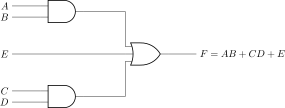
\includegraphics[width=234.0pt]{lect_3_two_level_sop}\caption{AND--OR}
\end{subfigure}
\\[6pt]
\begin{subfigure}[b]{236.0pt}\centering
  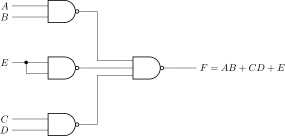
\includegraphics[width=234.0pt]{lect_3_two_level_sop_nand}\caption{NAND--NAND}
\end{subfigure}
\\[6pt]
\begin{subfigure}[b]{247.6pt}\centering
  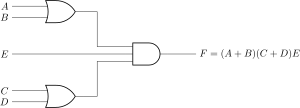
\includegraphics[width=245.6pt]{lect_3_two_level_pos}\caption{OR--AND}
\end{subfigure}
\caption{Two-level circuits: an SOP as AND--OR and as NAND--NAND (a, b); a POS as OR--AND and as NOR--NOR (c, d).}\label{fig:twolevel}
\end{figure}

\begin{figure}[htbp]
\centering
\ContinuedFloat
\begin{subfigure}[b]{247.6pt}\centering
  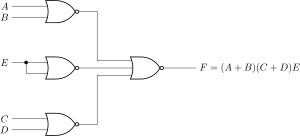
\includegraphics[width=245.6pt]{lect_3_two_level_pos_nor}\caption{NOR--NOR}
\end{subfigure}
\caption[]{Two-level circuits: an SOP as AND--OR and as NAND--NAND (a, b); a POS as OR--AND and as NOR--NOR (c, d).}
\end{figure}

\section{Exclusive-OR and Exclusive-NOR}
The \term{exclusive-OR} (XOR) function is 1 when its inputs \emph{differ}: $x\xor y = x'y+xy'$. The \term{exclusive-NOR} (XNOR, or \emph{equivalence}) is 1 when the inputs are \emph{equal}: $(x\xor y)' = xy+x'y'$. Both are fundamental in arithmetic and comparison circuits. Useful identities are
\[
 x\xor 0 = x,\qquad x\xor 1 = x',\qquad x\xor x = 0,\qquad x\xor x' = 1,
\]
and XOR is commutative and associative, $A\xor B = B\xor A$ and $(A\xor B)\xor C = A\xor(B\xor C)$, so that XOR of more than two variables is unambiguous. The symbols are shown in \cref{fig:xor}.

\begin{figure}[htbp]
\centering
\begin{subfigure}[b]{144.7pt}\centering
  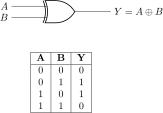
\includegraphics[width=142.7pt]{lect_3_xor_symbol}\caption{XOR}
\end{subfigure}
\hfill
\begin{subfigure}[b]{144.7pt}\centering
  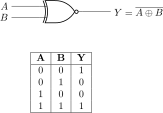
\includegraphics[width=142.7pt]{lect_3_xnor_symbol}\caption{XNOR}
\end{subfigure}
\caption{Symbols and truth tables of XOR and XNOR.}\label{fig:xor}
\end{figure}

\subsection{Odd and even functions}
The XOR of several variables is 1 when an \emph{odd} number of its inputs are 1; it is called the \term{odd function}. Its complement, the XNOR of several variables, is 1 when an \emph{even} number of the inputs are 1, and is called the \term{even function}. On a K-map these functions have a checkerboard pattern in which no two 1s are adjacent, so no simplification is possible (\cref{fig:oddeven}). For three variables
\[
 A\xor B\xor C = \Sm(1,2,4,7), \qquad (A\xor B\xor C)' = \Sm(0,3,5,6).
\]

\begin{figure}[htbp]
\centering
\begin{subfigure}[b]{183.5pt}\centering
  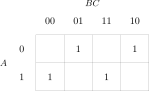
\includegraphics[width=181.5pt]{lect_3_kmap_odd}\caption{K-map of the odd function $A\xor B\xor C$}
\end{subfigure}
\hfill
\begin{subfigure}[b]{173.5pt}\centering
  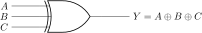
\includegraphics[width=171.5pt]{lect_3_logic_odd}\caption{logic diagram of the odd function}
\end{subfigure}
\\[6pt]
\begin{subfigure}[b]{183.5pt}\centering
  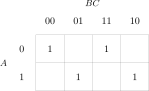
\includegraphics[width=181.5pt]{lect_3_kmap_even}\caption{K-map of the even function $(A\xor B\xor C)'$}
\end{subfigure}
\hfill
\begin{subfigure}[b]{173.5pt}\centering
  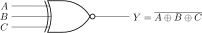
\includegraphics[width=171.5pt]{lect_3_logic_even}\caption{logic diagram of the even function}
\end{subfigure}
\caption{Odd and even functions of three variables: K-maps and logic diagrams.}\label{fig:oddeven}
\end{figure}

\section{Application: Parity Generation and Checking}\label{sec:parity}
XOR gates are ideal for detecting errors in data transmission. A \term{parity bit} is an extra bit appended to a message so that the total number of 1s is always even (\term{even parity}) or always odd (\term{odd parity}). \Cref{fig:parity-system} shows the system: a parity generator at the transmitter, the channel, and a parity checker at the receiver.

\figside{481.9pt}{lect_3_parity_system}{A parity system: the generator appends a parity bit; the checker at the receiver signals an error.}{fig:parity-system}

\paragraph{Even-parity generator.} For a 3-bit message $x,y,z$ the parity bit $P$ must make the number of 1s in $(x,y,z,P)$ even. This is true if and only if $P$ is the odd function of the message: $P=x\xor y\xor z$.

\paragraph{Even-parity checker.} The receiver computes $C = x\xor y\xor z\xor P$ from the four received bits; $C=0$ means that the number of 1s is even and no error is detected, whereas $C=1$ signals an error. A single-bit error always changes the parity and is detected; a double-bit error is not.

\begin{figure}[htbp]
\centering
\begin{subfigure}[b]{261.7pt}\centering
  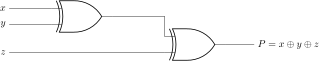
\includegraphics[width=259.7pt]{lect_3_logic_parity_generator}\caption{generator $P=x\xor y\xor z$}
\end{subfigure}
\\[6pt]
\begin{subfigure}[b]{320.8pt}\centering
  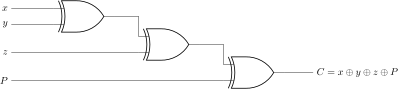
\includegraphics[width=318.8pt]{lect_3_logic_parity_checker}\caption{checker $C=x\xor y\xor z\xor P$}
\end{subfigure}
\caption{Even-parity generator and checker for a 3-bit message.}\label{fig:parity}
\end{figure}

\begin{lstlisting}[caption={Even-parity generator and checker in VHDL.},label={lst:parity}]
library ieee;
use ieee.std_logic_1164.all;

entity parity_generator is
  port (x, y, z : in  std_logic;
        p_even  : out std_logic);          -- parity bit for the even-parity scheme
end parity_generator;

architecture behavioral of parity_generator is
begin
  p_even <= x xor y xor z;                 -- 1 if the message has an odd number of 1s
end behavioral;

library ieee;
use ieee.std_logic_1164.all;

entity parity_checker is
  port (x, y, z, p_in : in  std_logic;     -- message and received parity bit
        err           : out std_logic);    -- 0 = no error detected, 1 = error detected
end parity_checker;

architecture behavioral of parity_checker is
begin
  err <= x xor y xor z xor p_in;           -- 1 if the total number of 1s is odd
end behavioral;
\end{lstlisting}

\begin{chaptersummary}
\begin{itemize}
  \item A \textbf{Karnaugh map} is a truth table arranged in Gray-code order so that adjacent squares differ in one variable. Groups of $2^k$ adjacent 1s eliminate $k$ variables.
  \item Group the 1s with \textbf{rectangles of size $2^k$}, as large as possible, allowing overlap and wrap-around; find all \textbf{prime implicants}, take the \textbf{essential} ones, then complete the cover with as few others as possible. A minimal SOP is not always unique.
  \item \textbf{Don't-cares} may be treated as 1 or as 0 to make larger groups.
  \item For a \textbf{minimal POS}, group the 0s and write sum terms (or simplify $F'$ and apply De~Morgan).
  \item \textbf{NAND} and \textbf{NOR} are universal; an SOP maps to a two-level \textbf{NAND--NAND} circuit, a POS to a two-level \textbf{NOR--NOR} circuit.
  \item \textbf{XOR} is the odd function and \textbf{XNOR} the even function; they form a checkerboard on the K-map and are the basis of \textbf{parity} generation and checking.
\end{itemize}
\end{chaptersummary}

\chapsec{Exercises}
\begin{exlist}
  \item Simplify $F(A,B,C)=\Sm(0,2,3,4,6)$. (a)~Construct the truth table. (b)~Draw the K-map and the groups. (c)~Write the minimal SOP. (d)~Draw the circuit with AND, OR and NOT gates.
  \item Simplify $F(w,x,y,z)=\Sm(0,1,2,7,8,9,10,15)$ with don't-cares $d(5,13)$. (a)~Draw the K-map, marking X squares. (b)~Find the minimal SOP, stating which don't-cares were used as 1s. (c)~Draw the circuit.
  \item Simplify $F(x,y,z)=\Sm(0,1,2,5,7)$ to a minimal \emph{POS}. (a)~Draw the K-map and plot the 0s. (b)~Find the minimal POS. (c)~Draw the two-level NOR--NOR circuit.
  \item \textbf{Prime and parity detector.} Design a 4-input circuit with inputs $A,B,C,D$ (binary number $ABCD$, $A$ the most significant bit) and two outputs. $F=1$ only when the input is a \emph{prime number} (0 and 1 are not prime). $G=1$ only when the number of 1s in the input is \emph{even}. Inputs 10--15 are not valid BCD and are don't-cares. (a)~Make one truth table for both outputs. (b)~Find the minimal SOP for $F$ and the minimal POS for $G$. (c)~Draw $F$ using only NAND gates and $G$ using only NOR gates.
  \item Find all prime implicants and all essential prime implicants of $F(w,x,y,z)=\Sm(0,2,3,5,7,8,10,11,13,15)$. Give all minimal SOP expressions.
  \item Simplify the following four-variable functions to minimal SOP: (a)~$F=\Sm(0,2,8,10)$; (b)~$F=\Sm(0,1,2,3,12,13,14,15)$; (c)~$F=\Sm(0,2,5,7,8,10,13,15)$.
  \item Convert the expression $F=AB+CD'+A'C'$ into (a)~a circuit with only NAND gates and (b)~a circuit with only NOR gates. Count the gates in each case.
  \item Show that the XOR operation is associative, $(A\xor B)\xor C = A\xor(B\xor C)$, by means of a truth table. How many 1s does the K-map of the 4-variable odd function $A\xor B\xor C\xor D$ contain?
  \item Design an \emph{odd}-parity generator for a 4-bit message $w,x,y,z$. Write the VHDL entity and architecture, and give the output for the messages \bin{0110}, \bin{0111} and \bin{1111}.
  \item The 7-bit ASCII code of the letter `A' is \bin{1000001}. What parity bit must be appended for (a)~even parity and (b)~odd parity? A receiver using even parity gets \bin{11000001} (parity bit first): is an error detected? Can the receiver tell which bit is wrong?
  \item Complete the 4-bit BCD to seven-segment decoder of Exercise~2.4 by finding minimal SOP expressions for segments $b$ and $c$ with the help of K-maps (outputs for inputs 10--15 are don't-cares).
\end{exlist}

\chapsec{Further Reading}
Karnaugh's original paper~\cite{karnaugh1953} is short and clear. McCluskey's tabular method~\cite{mccluskey1956} is the basis for computer-aided minimisation, and is covered in most digital-design textbooks, including Mano and Ciletti~\cite{mano2018} and Wakerly~\cite{wakerly2006}, the latter with an excellent discussion of timing hazards in two-level logic. Brown and Vranesic~\cite{brown2009} treat minimisation, NAND/NOR implementation and multilevel synthesis in depth.
